\chapter{Results}
\label{chapter:Results}


\section{Using graph convolution in the way it's meant to be used gives poor results on molecular structures}
\label{sec:neighborhood-expansion}

In the paper Chen et al.~\cite{Chen2019} at Tencent Lab, the authors modify a well performing GCNN architecture for quantum chemistry invented by Gilmer et al.~\cite{Gilmer2017}. The authors expand this model by using both, categorical bond type and euclidean distance as edge features and observe considerably better performance. At first glance, the use of both kinds of features - which seems to be implied in the paper - looks like a plausible explanation for the success. However, upon closer inspection, the reasoning does not add up. Bond types almost completely determine the euclidean distance. E.g. ever carbon-carbon single bond has a distance of 154Å, every carbon-oxygen double bond is 120Å long, etc.~\footnote{\url{https://courses.lumenlearning.com/suny-potsdam-organicchemistry/chapter/1-3-basics-of-bonding}} (The same applies to the reverse: knowing the distance between two atoms as well as the atom types allows to deduce the type of covalent bond or lack thereof.) Therefore, no additional information is added by including the euclidean distance as a feature. Inspection of the implementation reveals anther possible reason for the good performance of the Tencent Lab-paper: Not only is the euclidean distance added as a feature to existing edges, every atom is connected to every other atom in the molecule with the euclidean distance being the only not-null feature~\footnote{\url{https://github.com/tencent-alchemy/Alchemy}}. Thus, the structure of the graph is changed dramatically form the graph of covalent bonds to complete graph where every node is connected to every other node. The complete graph is a special case of graph and is rather untypical because in most applications, the presence or absence of an edge between two nodes is the most important kind of information. Simply connecting all nodes with each other seems to diminish this information (although in this case, the euclidean distance allows to distinguish between important and less important edges). With these considerations it is surprising but very interesting that the approach of Tencent Labs works so well.

In preparation for this thesis, I participated in the Tencent-Alchemy competition~\footnote{\url{https://alchemy.tencent.com}} using approach described above a baseline architecture. Despite many experiments, I achieved the best results simply fine-tuning Tencent Labs model and finished 26th out of 53 participants. The fact that half the participants did not beat the baseline published in the official competition paper, shows that the approach is indeed quite effective an warrants a closer examination why the peculiar approach of using complete graphs works quite well.

%As discussed in the introduction, a central concept of graph convolution (and regular convolution as well), is to compute a representation of a local neighborhood. In the case of graphs, a local neighborhood is a node and its neighbor nodes while on images, it is a small patch of pixels, such as 3x3 or 5x5.


As explained in the introduction, we can define the neighborhood of a node as all other nodes within a certain distance threshold. We refer to this threshold as neighborhood radius.

Therefore, the first experiment, we compare the learning curves of graphs when defining the neighborhood with different thresholds. First of all, covalent bonds are always represented as edges in the graph. Then, for increasing radii, edges to all non-covalently bonded atoms within the radius are added to the graph. A neighborhood radius of zero thus means that no additional edges are added to the graph - the graph only has edges between covalently bonded atoms. At a radius of 1.5 Ångström (1Å = 10nm), an edge is added between any two non-covalently bonded atoms with a distance of at most 1.5Å. The same is done for 2Å, etc. For perspective, most covalent bonds in organic molecules have a distance of around 1 - 1.5 Å~\footnote{\url{https://courses.lumenlearning.com/suny-potsdam-organicchemistry/chapter/1-3-basics-of-bonding}}. 1.5Å is very close for non-covalently bonded atoms such that only very few non-covalently bonded atoms - if any - will be within 1.5Å of an atom in an organic molecule. With a 2Å radius, every atom in the molecule will get some new neighbors due to this rule. With a 4Å radius, many atoms will be included in the neighborhood that have very little to no interaction with the central atom. At 5Å, for many small molecules, every atom is considered a neighbor of any other atom - applying this radius is therefore similar to connecting every atom with every other atom in the molecule. Finally, with an infinite radius, a complete graph is obtained.

\begin{figure}[H]
	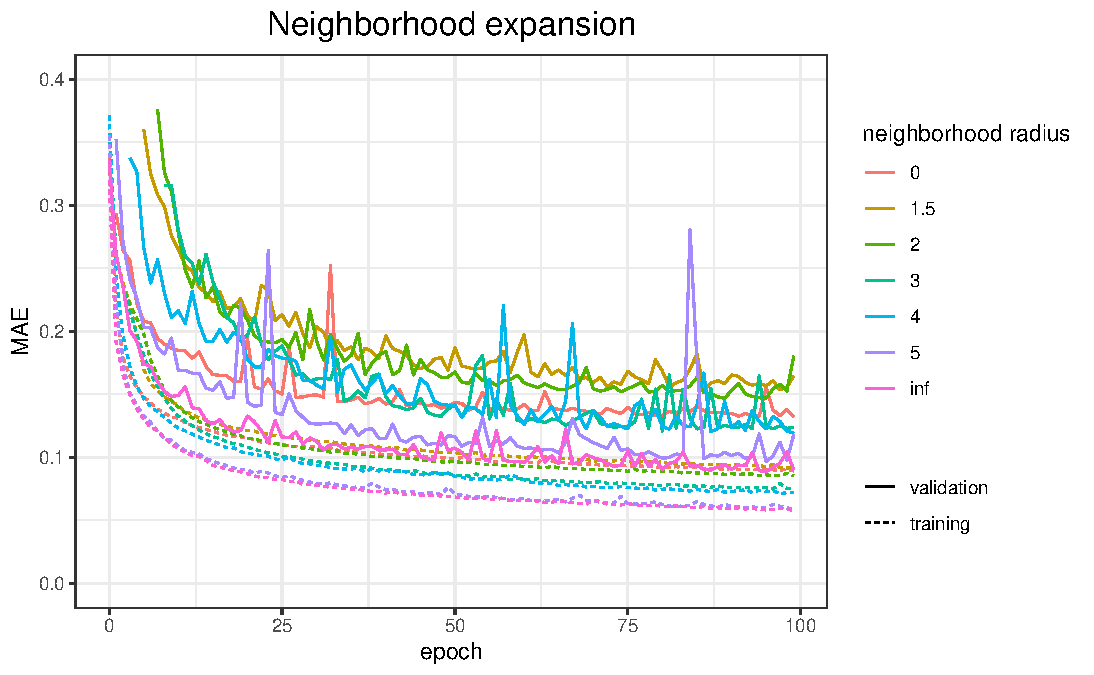
\includegraphics[width=\linewidth]{figures/tencent-mpnn-neighborhood-expansion-old}
	
	\caption{The learning curves with different neighborhood radii are show over the courses of 100 epochs. The color corresponds to the neighborhood radius, dotted lines the training errors and solid lines show validation errors. Note that for each radius, there is a training- and a validation-error curve. Each curve is an average of three learning curves with the same neighborhood radius. All curves were generated using a simple optimization scheme described in Section~\ref{sec:training}. Both, validation- and training-error could be lowered considerably by employing a more sophisticated optimization scheme. However, this would be at the expense of comparability between curves (see Section~\ref{sec:training}).}
	\label{fig:tencent-mpnn-neighborhood-expansion}
\end{figure}

As Figure~\ref{fig:tencent-mpnn-neighborhood-expansion} shows, the best performance is indeed achieved with the complete graph - connecting every atom with every other atom in the molecule with an edge. In general, the larger the neighborhood radius, the better the performance~\footnote{Exception: radius 0}. This result is in line with the suspicion that the real reason for the good performance of Tencent Lab's model is the addition of new edges rather than the addition of the euclidean distance feature.
The result is somewhat counterintuitive and in contrast with the principle of (graph-)convolution. As described in the introduction, in theory, graph convolutions update node-representation based on the local neighborhood of each node. Eventually, after $t$ layers, each node representation would contain indirect contributions from all other nodes with $t$ or less edges between. However, the results shown here show that the performance is best if the graph convolution considers all atoms at every layer. This contrast clearly shows that much remains to be discovered about the use of GCNN for molecules.

For small molecules and with considerable computational power at hand, one could simply accept this finding as it is and represent molecules as complete graphs. However, for larger molecules with hundreds of atoms, this would be computationally not feasible as the number of edges increases quadratically ($\frac{n(n - 1)}{2}$ edges for $n$ nodes). Therefore, further experiments will aim at finding an alternative way that captures the advantage of the complete graph-approach without the excessively high computational cost.

%Emphasize that this is not really appreciated in the literature.
%Cite Alchemy paper and point out that the high-performing kaggle-teams all use fully connected graphs.
%Does no one notice?


\section{Introducing a graph-state at every graph-conv layer improves results}


What the usage if complete graphs in graph convolutional networks essentially does is that it ensures that during every node update, a representation of every other node in the graph contributes to the update - even nodes that are too far away to have any direct interaction with the updated node (atom).
A possible explanation of this behavior is that the node update benefits from having access to information about the whole graph / molecule. This interpretation begs the question if a similar effect can be achieved by a different architecture (that does not require the use of computationally prohibitive complete graphs).

An interesting experiment to test this hypothesis is to include graph-level information at every node update (without having to use complete graphs.) One such idea is the use of a root node. A root node is a virtual node that is connected to every other node in the graph. In the molecule case, the root node does not represent a real atom. Instead, it can be used to represent information about the whole molecule. Then, as every node is connected to the root node, every node update has access to information about the whole molecule. On could initialize the root node representation with molecule level features (such as number of atoms, electric dipole, etc.[CITATION]). However, all those features are implicit in the 3D molecular structure. Sticking to the pure deep learning philosophy, the root node representation can also be learned solely from the raw data.

Ideally, the use of such a root node would allow to achieve a similar performance as when using complete graphs without the high computational cost - while the number of edges increases quadratically with the number of nodes in the complete graph, the root node only introduces one new edge per node. At the very least, the effect of of decreasing performance with decreasing neighborhood radius shown in Figure~\ref{fig:tencent-mpnn-neighborhood-expansion} should be less pronounced if the root node has the expected effect.






\section{Manual feature engineering does not improve prediction accuracy.}

% compare raw vs. tencent features.
% after the point has been made, use only raw data

\section{Excluding hydrogen atoms from the molecule-graph speeds up training but reduces prediction accuracy}

Another possible preprocessing step is to disregard hydrogen atoms and instead add the number of hydrogen atoms bonded to a given heavy atom as a node feature. The rational behind this step is that the properties chemical properties of hydrogen atoms depend strongly on the heavy atom to which it is bound. While some information is lost during this step, the number of atoms in the molecule is reduced by an average factor of [CHECK value]. This modest reduction in the number of nodes leads to a very dramatic reduction in the number of edges. Naturally, this effect is most pronounced in complete graphs where the number of edges increases quadratically with the number of nodes ($\frac{n(n - 1)}{2}$ edges for $n$ nodes). While the average number of edges using complete graphs is [CHECK value] in the AlChemy dataset, this number drops to [CHECK value] after excluding hydrogen atoms.

The approach of not considering hydrogen atoms explicitly but only as features of heavy atoms is known as using \textit{implicit hydrogen atoms}. In short, it is a way of summarizing raw data which speeds up training considerably while loosing some information. Figure [] shows...

% probably: larger error
% => use explicit hydrogen atoms from now on


\section{graph-conv layers with independent weights decrease the loss slightly}


In most graph neural networks, the graph-conv layers have shared weights. This allows for efficient training and works well in practice. However, there is no theoretical reason that weight sharing is necessarily superior. For instance, it would be conceivable that independent weights would work better for extracting different kinds of features at each graph-conv step. Recall that the graph-conv layer, the input for a given node update consists only of direct neighbor nodes, at the second layer, the update indirectly contains information from all second-degree neighbor nodes etc. Hence, learning different weights for different graph-conv layers might be beneficial. Note also that in computer vision every layer has independent weights even within blocks of convolutional layers with the same dimension. It is therefore far from clear that weight sharing has to be the preferred approach for graph-conv layers.

In order to investigate the possible benefit of independent weights, the next experiment compares the MPNN described in previous section with an architecture without weight sharing. The two architectures are identical in every other aspect to allow isolate the effect of weight sharing. Figure~\ref{fig:weight-sharing} shows a small but not negligible advantage of the net using independent weights in the graph-conv layers. Another interesting observation is that the learning curves are almost identical apart from the lower MAE of the model with independent weights. It would not have been surprising for the independent weights to require more training time as each graph-conv layers weights are only updated once for a given batch in a given epoch. In weight-sharing architectures on the other hand, the conv-layer is updated $n$ times for each batch and epoch in a model with $n$ conv-layers. Nevertheless, Figure~\ref{fig:weight-sharing} clearly shows that the two approaches are equal in terms of training-time. This means that the use of independent weights is a simple way to gain a small improvement sacrificing efficiency.

One caveat worth mentioning is that only because independent weights were found to be beneficial for the architecture at hand does not mean that they will be beneficial in every single graph-conv net. However, the results at hand make a strong case for independent weights as a way to improve the performance of graph convolutional networks. 



\begin{figure}[H]
	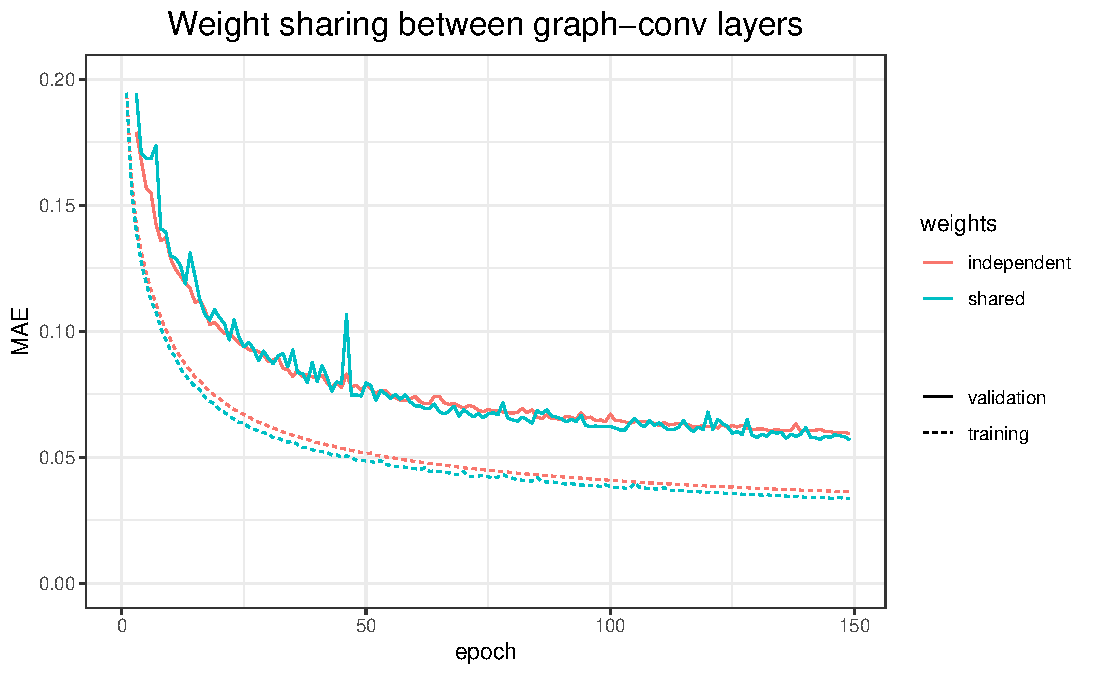
\includegraphics[width=\linewidth]{figures/weight-sharing.pdf}
	
	\caption{Independent weights between graph-conv layers outperform weight-shared layers by a small margin. Note that the two architectures are identical in every other way apart from weight-sharing of graph-conv layers. Complete graphs were used as the input data as this was shown to be the best performing transformation in earlier experiments (Section~\ref{sec:neighborhood-expansion}). Importantly, each learning curve in this figure represents an average over three independently trained model to minimize the influence of random fluctuations between training-runs. The learning rate was set to a start value of $0.001$ with a learning rate decay of 0.99 each epoch. While a more sophisticated optimization scheme and training for more epochs could have given slightly a somewhat lower MAE, the results a at hand show clearly the relative advantage of independent weights.}
	\label{fig:weight-sharing}
\end{figure}

\section{relative position edge features improve results slightly}

{\itshape
 Show that relative position edge features slightly improve the results but not much
 
 explain that the problem is probably that they are not rotation-invariant
	
	
OPTIONAL PART:\\
review the results of the 3DGCN-paper and show that this doesn't work really well on the Alchemy data - probably for the same reason given above
}






